\chapter{Dettagli}
\label{dettagli}

In questo capitolo si trattano i dettagli implementativi relativi alle modifiche operate a:
\begin{itemize}
	\item Una variante della libreria FIDO2 realizzata da Yubico modificata in una tesi precedente per accogliere il meccanismo survivable \cite{yubico:fido}
	\item Il codice sorgente dell'autenticatore Solokeys \cite{solokeys:code} per integrare il \emph{security level}
\end{itemize}

Nonostante la libreria Yubico fosse già stata modificata in precedenza per adottare la struttura survivable, è stato comunque necessario operare cambiamenti. La libreria FIDO2 si occupa di simulare l'interazione tra un Client FIDO2 e un Server FIDO2 per emulare la registrazione e la successiva autenticazione. Grazie alla modifica apportata precedentemente è possibile simulare un numero arbitrario di Server con cui stabilire la comunicazione e svolgere tali operazioni. Tutto il funzionamento descritto nel capitolo precedente è correttamente gestito, ad esclusione dell'invio del security level.

Lato autenticatore invece si è reso necessario implementare diverse funzionalità: dal parsing del security level nel messaggio inviato dall'User Agent all'autenticatore fino ad arrivare a un contatore globale vero e proprio. Infatti, da standard FIDO2 il signature counter utilizzato per il controllo della clonazione dell'autenticatore può essere anche globale e non specifico per credenziale \cite{fido:signature_counter}. Ciò è dovuto alla natura \emph{constraint}, cioè con limitazioni di memoria importanti, degli autenticatori hardware.

\section{Modifica della libreria FIDO2}
\label{modifica_fido}

La libreria FIDO2 presenta il file \verb*|client_multichallenge.py| in cui viene definita la classe \verb*|Fido2ClientMultichallenge|, figlia della classe \verb*|Fido2Client| nel relativo \verb*|client.py|, che permette l'autenticazione WebAuthn simulando un Client FIDO. Presenta due metodi, \verb*|make_credential| per realizzare l'operazione di creazione delle credenziali e \verb*|get_assertion| per compiere l'operazione di autenticazione. 

Rispetto alla condizione di partenza è stato aggiunto il controllo del contatore lato server. Per fare ciò è stato definito all'interno del costruttore di \verb*|Fido2ServerMultichallenge| un dizionario tramite cui tenere traccia dei contatori:
\begin{verbatim}
	self.counter_register = {}
\end{verbatim}
I metodi interessati della classe sono sostanzialmente due: 
\begin{itemize}
	\item \verb*|register_complete|
	\item \verb*|authenticate_complete|
\end{itemize}

Entrambe le funzioni si occupano di controllare la correttezza dei dati ricevuti dal Client dopo che ha interpellato l'autenticatore. Entrambi i metodi vengono chiamati nel file \verb*|client_multichallenge.py| e ad entrambi è stato aggiunto il passaggio del parametro \verb*|security_level|.

Nel primo metodo, \verb*|register_complete|, viene salvato il contatore ricevuto all'interno del dizionario. Per fare ciò viene creato un secondo dizionario interno al primo, utilizzando il \emph{CredentialID} ricevuto in dall'autenticatore. In questo secondo dizionario sarà presente la coppia \verb*|security_level|:\verb*|contatore|. 
\begin{verbatim}
self.counter_register[credential_id] 
    = 
      {security_level: attestation_object.auth_data.counter}
	
\end{verbatim}

Nel secondo metodo invece vengono effettuati i controlli sulla base di quanto salvato dal server nel proprio dizionario e quanto ricevuto dall'autenticatore. In caso di contatore ricevuto minore o uguale a quello immagazzinato viene sollevato un errore che porta alla terminazione del programma. 
\begin{verbatim}
	if auth_data.counter <= self.counter_register[credential_id][security_level]:
	    raise ValueError("Counter did not increase.")
\end{verbatim}
Questo perchè si suppone che vi sia stato un tentativo di clonazione. 

Qualora, invece, il contatore fosse maggiore di quello immagazzinato $+1$ allora verrà solamente notificato il fornitore del server tramite un messaggio in console di log. 
\begin{verbatim}
elif auth_data.counter > self.counter_register[credential_id][security_level] + 1:
    print("Counter bigger than expected")
\end{verbatim}
In quest'ultimo caso e nel caso in cui il contatore venga incrementato correttamente viene aggiornato il valore corrispondente nel dizionario del server. Se nessuna di queste condizioni è verificata vuol dire che non è presente nel dizionario una voce con quel dato security level: in questo caso viene semplicemente aggiunto il security level al dizionario interno con il relativo contatore.

\begin{verbatim}
	self.counter_register[credential_id][security_level] = auth_data.counter
\end{verbatim}

\begin{center}
	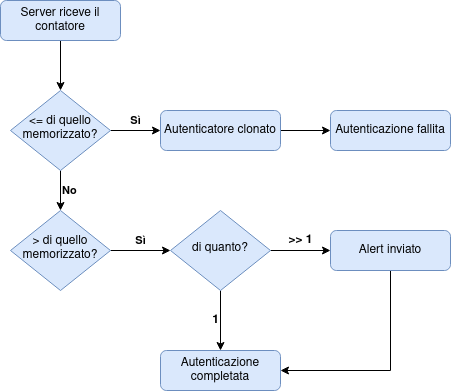
\includegraphics[width=.6\columnwidth]{figures/flowchart_contatore}
	\label{fig:contatore_webauthn}
\end{center}

\section{Modifica del codice Solo}
\label{modifica_solo}

Il codice dell'autenticatore Solokeys, come detto in precedenza, presentava un solo contatore globale per tenere traccia di tutte le operazioni di creazione/autenticazione svoltesi con successo. Il primo passo è stato, quindi, quello di implementare una struttura dati per la memorizzazione di un contatore per credenziale. Tale struttura dati, definita \verb*|signCounter| è una tipo di dato composto da due valori.
\begin{itemize}
	\item Una istanza \verb*|id| della \emph{struct} \verb*|CredentialId|
	\item Un intero senza segno di 32 bit definito come \verb*|signCount|
\end{itemize}

La struttura dati \verb*|CredentialId| definisce come vengono memorizzate le credenziali all'interno dell'autenticatore seguendo lo standard FIDO \cite{fido:credential_id}. In particolare, invece che avere una sequenza di 16 bytes come da standard, presenta valori come \begin{verbatim}
	tag, nonce, padding, metadata, rpIdHash
\end{verbatim} 

La definizione della struttura \verb*|signCounter| è effettuata all'interno del file \verb*|ctap.h| e sempre nello stesso file è inizializzato anche \verb*|signCounterArray|, cioè un array di strutture dati \verb*|signCounter|. Tramite questo array è possibile memorizzare un contatore per credenziale. 

L'array viene popolato nel momento in cui viene chiamata la funzione \verb*|ctap_make_credential| utilizzata dall'autenticatore per compiere le operazioni di creazione delle credenziali. In particolare:
\begin{itemize}
	\item tramite un intero senza segno \verb*|globalCounter| viene tenuta traccia dell'ultima posizione dell'array occupata
	\item viene istanziata una struttura dati \verb*|signCounter| con \verb*|id| pari a quello calcolato e $\verb*|signCount| = 1 $
	\item viene aggiunta la struttura dati \verb*|signCounter| all'array \verb*|signCounterArray| alla posizione \verb*|globalCounter|
\end{itemize}

Nel momento in cui viene chiamata la funzione \verb*|ctap_get_assertion| viene cercata iterativamente la struttura dati il cui \verb*|id| corrisponde a quello dell'operazione corrente e viene incrementato il contatore di tale struct. 

\begin{verbatim}
    for (uint l = 0; l <= globalCounter; l++) {
        if (count_cmp_func(&cred->credential.id, &signCounter1[l])) {
            count = update_sign_counter(&signCounter1[l], GA.securityLevel);
        }
    }
\end{verbatim}

Per verificare che l'\verb*|id| corrisponda a quello generato in fase di \verb*|get_assertion| è stato necessario scrivere una funzione di comparazione: il C, infatti, non supporta nativamente la comparazione di due struct. A tal scopo è stata scritta la funzione \verb*|count_cmp_func| che compara attributo dopo attributo tutti quelli presenti all'interno della struttura per verificarne l'uguaglianza.
Il contatore, invece, viene aggiornato tramite la funzione \verb*|update_sign_counter| che semplicemente prende il valore \verb*|signCount| passato in chiamata e restituisce $signCount + 1$.

Il passo successivo è stato quello di modificare la struttura dati \verb*|signCounter| per fare in modo che accogliesse un contatore per \emph{security level}. Per fare ciò l'attributo \verb*|signCount| è stato cambiato da intero senza segno di 32 bit ad array di interi senza segno di 32 bit. Analogamente al processo di incremento seguito prima, il contatore corrispondente al security level ricevuto verrà aggiornato nel seguente modo:
\begin{verbatim}
	update_sign_counter(signCounter.signCount[n]])
\end{verbatim}
Così facendo vengono mantenuti e incrementati \emph{n} signature counter differenti per ogni credenziale. 


L'ultimo passaggio è stato quello di ricezione del \emph{security level}. Lo standard CTAP2 \cite{fido:ctap_commands} definisce i codici dei comandi a cui deve essere associato il lancio di alcune funzioni. Ogni comando è strutturato con il proprio codice di comando e i codici per i propri parametri. I codici per per i comandi di interesse sono i seguenti: 
\begin{verbatim}
	0x01	authenticatorMakeCredential
	0x02	authenticatorGetAssertion
\end{verbatim}


L'autenticatore Solo sfrutta il polling per controllare l'arrivo di messaggi da parte del Client. Al giungere di uno di questi viene controllato il codice del comando presente nei primi byte e viene invocata la funzione indicata dal codice e di cui è stato mostrato un esempio sopra. Tale funzione a sua volta effettuerà il parsing, cioè l'analisi del contenuto, per ottenere i parametri della funzione invocata. Oltre ai codici per i parametri già esistenti dei comandi \verb*|authenticatorMakeCredential| e \verb*|authenticatorGetAssertion| è stato necessario aggiungere nel file \verb*|ctap.h|:
\begin{verbatim}
	0x0A	MC_securityLevel
	0x08	GA_securityLevel
\end{verbatim}
Per definire i codici con cui codificare i livelli di sicurezza da usare, rispettivamente, in fase di creazione credenziali (\textbf{M}ake\textbf{C}redential) e autenticazione (\textbf{G}et\textbf{A}ssertion). 

Solo utilizza delle funzioni definite nel file \verb*|ctap_parse.c| per fare il parsing del flusso di dati CBOR ricevuto dal Client. In particolare sono presenti due funzioni:
\begin{itemize}
	\item \verb*|ctap_parse_make_credential|
	\item \verb*|ctap_parse_get_assertion|
\end{itemize}

che si occupano di controllare il flusso di dati per ottenere i parametri necessari alle funzioni \verb*|ctap_make_credential| e \verb*|ctap_parse_credential| per poter compiere le operazioni di creazione/autenticazione. In questo caso viene aggiunto allo \verb*|switch| l'identificazione dei codici definiti sopra per il parametro \emph{security level}. 

Di seguito il funzionamento semplificato all'interno della funzione \verb*|ctap_parse_make_credential|:
\begin{verbatim}
    switch(cmd)
    {
        ...
        case MC_securityLevel:
            cbor_value_get_int(MC->securityLevel)
        ...
    }
\end{verbatim}
La struttura dati \verb*|MC| rappresenta il risultato del parsing di tutti gli attributi nel flusso di dati ricevuto e viene restituita dalla funzione \verb*|ctap_parse_make_credential| al chiamante, in questo caso la funzione \verb*|ctap_make_credential|. In questo modo all'interno della funzione \verb*|ctap_make_credential|, dove si realizza l'inizializzazione della struttura dati \verb*|signCounter| e, conseguentemente del contatore \verb*|signCount|, è possibile utilizzare il valore del \emph{security level} ricevuto dal Client e incrementare di conseguenza il contatore corrispondente.

Analogo quanto avviene all'interno della funzione \verb*|ctap_parse_get_assertion| con la differenza che la struttura restituita alla funzione \verb*|ctap_parse_assertion|, cioè dove si realizza l'incremento del contatore, sarà chiamata \verb*|GA|.


\section{Testing}
\label{testing}

I test delle modifiche al codice Solo e alla libreria FIDO sono stati effettuati in locale. Per la parte di WebAuthn è stato utilizzato il file \verb*|client_multichallenge.py| che simula, utilizzando le classi \verb*|Fido2ClientMultichallenge| e \verb*|Fido2ServerMultichallenge|, la fase di creazione delle credenziali e poi l'autenticazione di queste con un numero arbitrario di FIDO Server operanti localmente. 
L'integrazione fatta al codice già presente è stata di definire i livello di sicurezza da utilizzare durante le due operazioni. 

Per quanto riguarda l'autenticatore, invece, è stato utilizzato un emulatore scritto da Solo che permette la simulazione di un autenticatore virtuale comunicante tramite protocollo UDP. Questo ha evitato di dover compiere le operazioni tipiche dei dispositivi embedded di \emph{flash} del software sull'autenticatore fisico e ha snellito sensibilmente il processo di test. 

Per fare in modo che l'emulatore UDP di Solo comunicasse con il Client FIDO2 della relativa libreria è stato necessario apportare delle modifiche alla classe \verb*|CtapHidConnection| che si occupa di definire, per i principali sistemi operativi, i metodi grazie ai quali è possibile interagire con gli \emph{Human Interface Device}. Per HID si intendono genericamente quei dispositivi elettronici che permettono l'interazione, sia essa in input o in output, con un essere umano. Gli autenticatori hardware fanno quindi parte degli HID. 
In particolare è stato aggiunto il file \verb*|udp_backend.py| in cui viene definita la classe \verb*|UdpCtapHidConnection| facendo l'override della classe \verb*|CtapHidConnection|. Nello specifico:
\begin{itemize}
	\item Viene definito un attributo della classe, chiamato \verb*|sock|, che rappresenta il \emph{socket} tramite cui avviene la comunicazione UDP
	\begin{verbatim}
		self.sock = socket.socket(socket.AF_INET, socket.SOCK_DGRAM)
	\end{verbatim}
	L'elemento fondante del protocollo UDP sono, infatti, i SOCKET, combinazioni di indirizzi IP e porte necessari per la comunicazione.
	\item Vengono ridefiniti i metodi di scrittura e lettura dei pacchetti utilizzando i metodi della libreria \verb*|socket| per l'invio e la ricezione tramite UDP
	\begin{verbatim}
        def write_packet(self, data):
            self.sock.sendto(data, self.remote)/CLionProjects/
		
        def read_packet(self):
            data, host = self.sock.recvfrom(self.descriptor.report_size_out)
        return data
	\end{verbatim}
\end{itemize}
Per realizzare questa modifica è stato integrato il codice già scritto da Solo per il proprio strumento di interazione a riga di comando con l'autenticatore \cite{solo1-cli:udp_backend}.